% Lower bound exponents for K_k detection: previous best and this work.
% Previous: k = 3 from [CGZ26], k >= 4 the larger of [GZ26] and the bound for K_{k-1}.
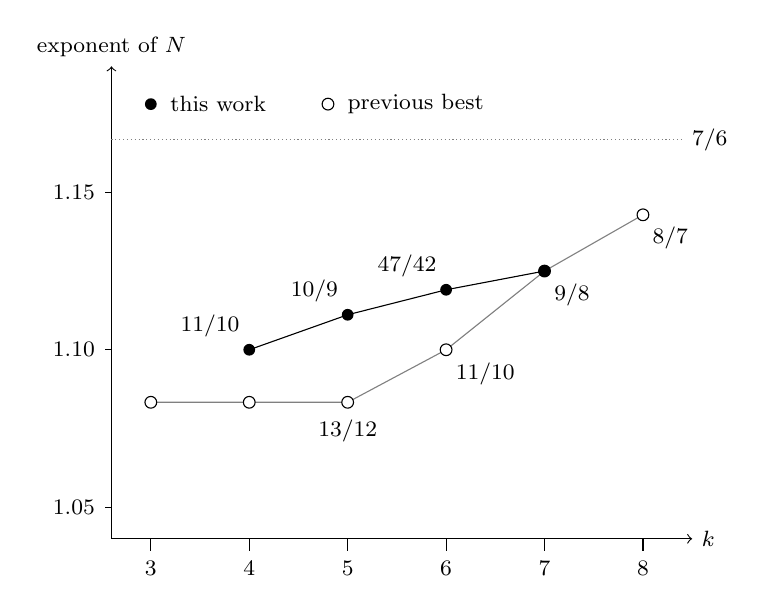
\begin{tikzpicture}[x=1.25cm,y=40cm,
  lab/.style={font=\footnotesize},
  old/.style={circle,draw,fill=white,inner sep=1.5pt},
  new/.style={circle,fill=black,inner sep=1.5pt}]
  \draw[->] (2.6,1.04) -- (8.5,1.04) node[lab,right] {$k$};
  \draw[->] (2.6,1.04) -- (2.6,1.19) node[lab,above] {exponent of $N$};
  \foreach \k in {3,...,8} {\draw (\k,1.04) -- (\k,1.036) node[lab,below] {\k};}
  \foreach \y/\t in {1.05/1.05,1.10/1.10,1.15/1.15} {\draw (2.6,\y) -- (2.53,\y) node[lab,left] {\t};}
  \draw[densely dotted,gray] (2.6,1.16667) -- (8.4,1.16667) node[lab,right,black] {$7/6$};
  % previous best: 13/12, 13/12, 13/12, 11/10, 9/8, 8/7
  \draw[gray] (3,1.08333) -- (4,1.08333) -- (5,1.08333) -- (6,1.1) -- (7,1.125) -- (8,1.14286);
  \foreach \k/\y in {3/1.08333,4/1.08333,5/1.08333,6/1.1,7/1.125,8/1.14286} {\node[old] at (\k,\y) {};}
  % this work: 11/10, 10/9, 47/42, 9/8
  \draw (4,1.1) -- (5,1.11111) -- (6,1.11905) -- (7,1.125);
  \foreach \k/\y in {4/1.1,5/1.11111,6/1.11905,7/1.125} {\node[new] at (\k,\y) {};}
  \node[lab,anchor=south east] at (4,1.101) {$11/10$};
  \node[lab,anchor=south east] at (5,1.112) {$10/9$};
  \node[lab,anchor=south east] at (6,1.120) {$47/42$};
  \node[lab,anchor=north] at (5,1.081) {$13/12$};
  \node[lab,anchor=north west] at (6,1.099) {$11/10$};
  \node[lab,anchor=north west] at (7,1.124) {$9/8$};
  \node[lab,anchor=north west] at (8,1.142) {$8/7$};
  % legend
  \node[new] at (3.0,1.178) {}; \node[lab,anchor=west] at (3.1,1.178) {this work};
  \node[old] at (4.8,1.178) {}; \node[lab,anchor=west] at (4.9,1.178) {previous best};
\end{tikzpicture}
